\evenchapter[Galigeo \ensg]{Galigeo}

\section{Présentation de l'entreprise}

\subsection{Généralités}

Galigéo est une société parisienne spécialisée dans le géomarketing. Créé en 2001, elle propose aux entreprises d’améliorer l’efficacité de tous leurs métiers grâce à ses logiciels combinant expertise cartographique et modélisation prédictive. Grâce à ses logiciels visualisant, analysant et agissant directement sur les bases de données opérationnelles (applications métier, BI, CRM, …). Galigeo permet aux utilisateurs de se focaliser sur leur métier (retail \footnote{A completer}, distribution, marketing, sécurité, …).

Historiquement pionnier de la location Intelligence, Galigeo a poursuivi son développement ses dernières années en ajoutant la composante prédictive dans ses suites logiciels, composante basée sur les techniques innovantes de Machine Learning et d’Intelligence Artificielle.

En utilisant son expertise cartographique et de modélisation prédictive, Galigeo poursuit son développement en mettant à disposition de ses clients, des logiciels simples d’usage, à très forte valeur ajoutée métier.

De 2001 à 2006, Galigeo se consacre aux développements de solutions intelligentes en géodécisionnel pour faire de l'analytique avancée à partir de cartes géographiques. De 2006 à 2011, elle développe sa première solution logiciel, Galigeo Enterprise, qui permet par la suite, grâce à un nouveau pôle Conseil, de proposer des services spécifiques métier et adapté à chaque client autour du géomarketing. A partir de cette date, Galigeo va voir sa croissance augmenter sur le marché international en s'associant à différents partenaires. A partir de 2017 et jusqu'à aujourd'hui, Galigeo a choisi d'ajouter à ses solutions une composante prédictive très demandé sur le marché.

L'entreprise compte aujourd'hui une cinquantaine de clients très divers, grandes enseignes commerciales, services publiques, industries, etc. Galigeo peut fournir des solutions logiciels standards pour permettre à n’importe quelle entreprise de générer des rapports de géomarketing en utilisant des données interne et des données générales fournies par Galigeo. Elle réalise également des projet plus spécifique, propre à des besoins bien déterminés qui permette alors à ces client d’avoir une vraie valeur ajoutée et un géomarketing efficace.

% Image of the offices
\begin{figure}[H]
    \centering
    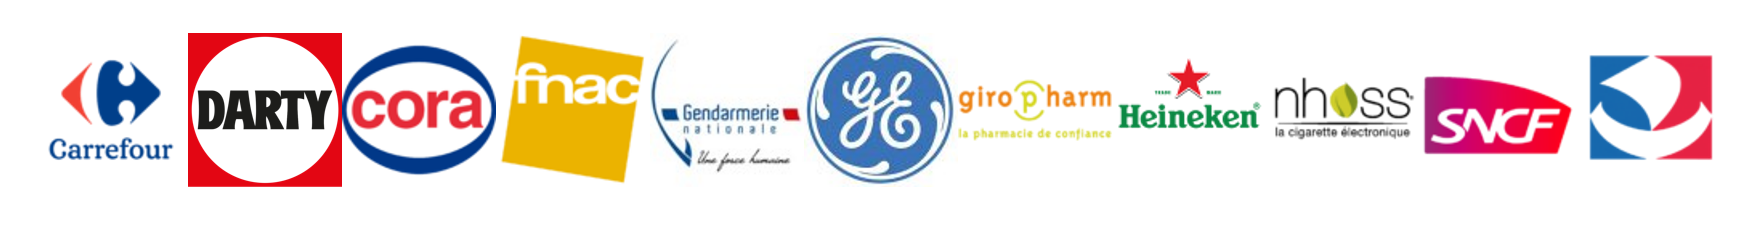
\includegraphics[width=\linewidth]{images/logos/client.png}
    \caption{Exemple de clients Galigeo}
    \label{fig:clients}
\end{figure}

Les bureaux de l'entreprise sont situé au 87 avenue d'Italie dans le treizième arrondissement de Paris.

% Image of the offices
\begin{figure}[H]
    \centering
    
\includegraphics[width=12cm]{images/photos/bureaux_galigeo.png}
    \caption{Bureaux de Galigeo, 87 avenue d'Italie, 75013 Paris}
    \label{fig:offices}
\end{figure}


\subsection{Organisation interne}

Galigéo est composé actuellement d’une vingtaine d’employés répartit dans 5 pôles : Administratif, Commercial, Marketing, Comptabilité, Consulting et Recherche et Développement.

Le pôle administratif est le pôle qui s’occupe de la gestion du budget, du personnel et des missions à Galigeo.

Le pôle commercial gère les relations clients, il propose des offres à de nouveaux ou ancien client, prospecte et cherche à faire grandir le cercle de clientèle de Galigeo.

Le pôle marketing imagine les produits, met en place les stratégies de pénétration du marché et réalise un catalogue de solutions que Galigeo peut fournir.

Le pôle comptabilité est responsable de la facturation des clients et la gestion interne des frais de personnels, des salaires, du matériel, etc.

Le pôle consulting est dédié à la réponse aux besoins techniques du client, il permet de rester proche du client. Il imagine les solutions retenues et les intègres dans les outils Galigeo mis à disposition pour l’entreprise.


Pour ma part, j’ai rejoint le pôle Recherche et Développement. L’équipe est composée de développeur, de testeurs, de designeur, de data scientist, etc. Elle s’attache à améliorer les produits de Galigeo et à faire du support, de la maintenance et de l’innovation. Lorsqu’un consultant est en charge d’un projet pour un client, il s’appuie sur un ou plusieurs membres de l’équipe R\&D pour conseiller ou réaliser les tâches techniques.

\paragraph*{}

J’ai principalement travaillé avec Raimana Teina, Data Sientist chez Galigeo autour du grand projet actuel chez Galigeo « Prédiction de flux piéton » que je détaillerais dans la suite de ce rapport. Cependant j’ai également eu l’occasion de travailler sur des projets clients avec l’équipe consulting.

% Image of the offices
\begin{figure}[H]
    \centering
    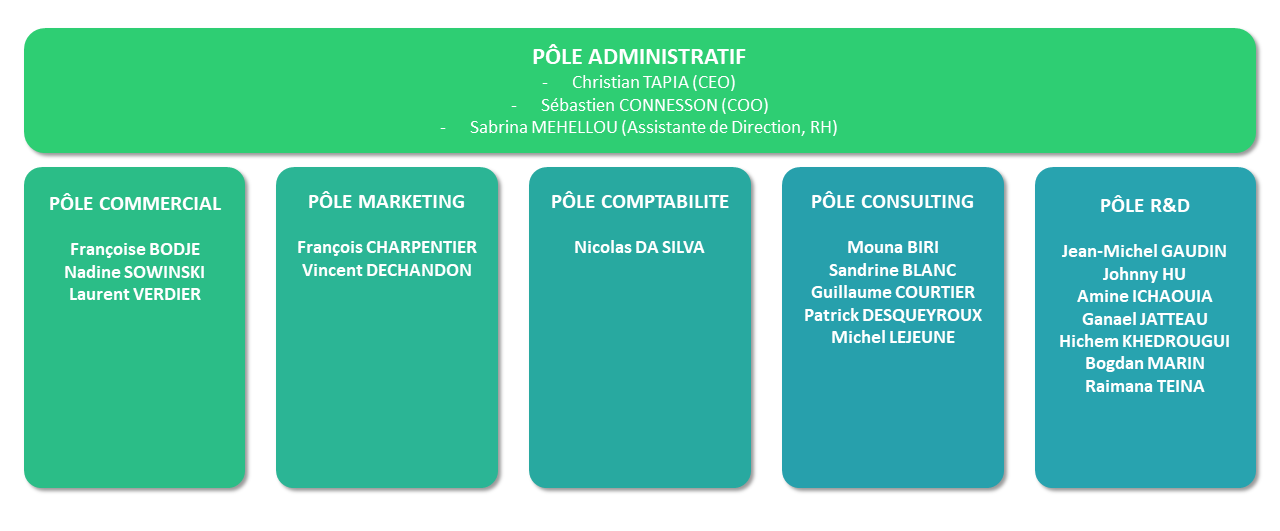
\includegraphics[width=\linewidth]{images/graphs/organigramme.png}
    \caption{Bureaux de Galigeo, 87 avenue d'Italie, 75013 Paris}
    \label{fig:organigrame}
\end{figure}


\section{Les objectifs de Galigeo}

\subsection{Les manques actuels}

Aujourd’hui, Galigeo cherche à mettre en avant des modèles prédictifs au service du géomarketing pour ses clients. Une mesure importante en géomarketing est l’estimation de flux piéton à un endroit donné et sur une période donnée. Jusqu’ici, Galigeo utilisait un service tier afin d’obtenir une estimation de flux piéton. Cette solution de transition possède néanmoins de nombreux défauts. Tout d’abord Galigeo n’avait aucune visibilité sur les algorithmes utilisés pour faire cette estimation.

Il était alors difficile d’utiliser les résultats de cette estimation dans l’entraînement de nouveaux modèles de prédiction (estimation de chiffre d’affaires, estimation de parts de marchés, etc.). De plus, les coûts d’une telle solution restent élevés.

Il a donc été décidé de créer un modèle d’estimation de flux piéton propre à Galigeo sur lequel l’entreprise aurait accès à toutes les données d’entrés du modèle. Ainsi elle pourra modéliser d’autre variables essentielles au géomarketing plus facilement et avec une meilleure qualité. En effet, en connaissance des biais de notre modèle, ils seront plus faciles à corriger dans d’autres cas d’utilisation.

Galigeo souhaite également renforcer son équipe big data afin de mettre en valeurs de grosse quantité de données brutes inexploitable en l’état. En recrutant de nouveaux data scientist, elle libèrera du temps à ses consultant et déchargera les équipes spécialisées dans la data actuellement en place.

\paragraph*{}

Après un entretien au printemps 2022 chez Galigeo et cette explication des manques et objectifs de l’entreprise à court termes, j’ai fait part de mon envie à réaliser un stage au sein de l’équipe R\&D. Ils ont retenu ma candidature et j’ai donc commencé mon stage de fin d’étude le 02 Mai 2022.


\subsection{Les objectifs du stage}

Durant ce stage j’avais donc comme première objectif de découvrir le géomarketing dans son ensemble. J’ai dû analyser et comprendre les cas d’usages métiers et me plonger dans le fonctionnement d’une équipe de développement logiciel.

J’avais également pour mission de concevoir et spécifier des solutions d’acquisition, de cleaning et de traitement des données. Comprendre le fonctionnement des produits Galigeo m’a permis de collecter et stocker la donnée de manière optimale afin de faciliter l’implémentation dans des bases de données.

J’avais également pour mission de développer des chaînes de collecte de la donnée en m’appuyant sur des méthodes de data engineering \footnote{A compléter}. Pour pouvoir par la suite utiliser au mieux la donnée dans des processus d’analyse et de traitement.

Pour la partie traitement de la donnée brute, mes objectifs étaient de développer des algorithmes et des traitements de la data grâce à des méthodes statistiques et de machine learning. Mon objectif était de transformer de la donnée brute inexploitable en une donnée pertinente pour le géomarketing des clients Galigeo.

\paragraph*{}

Mon objectif était également de m’intégrer aux équipes de Galigeo afin de mieux comprendre les objectifs de l’entreprise à long termes et les directions à prendre.


\subsection{Les objectifs à plus long termes}

\section{Organisation du stage}

\subsection{Planning}
\subsection{Mes missions}
\subsection{Relations internes et client}